\documentclass[a4paper,10pt]{article}
\usepackage[utf8]{inputenc}
\usepackage{amsmath}
\usepackage{amsfonts}
\usepackage{amssymb}
\usepackage{algorithm}
\usepackage[noend]{algpseudocode}
\usepackage{program}
\usepackage{amsmath}
\usepackage{graphicx}
\usepackage[T1]{fontenc}
\usepackage{eso-pic}
%\usepackage{gensymb}
\usepackage{listings}
\usepackage{float}

\newcommand\floor[1]{\lfloor#1\rfloor}
\newcommand\ceil[1]{\lceil#1\rceil}
\newcommand{\BackgroundPic}{\put(-4,0){\parbox[b][\paperheight]{\paperwidth}{\centering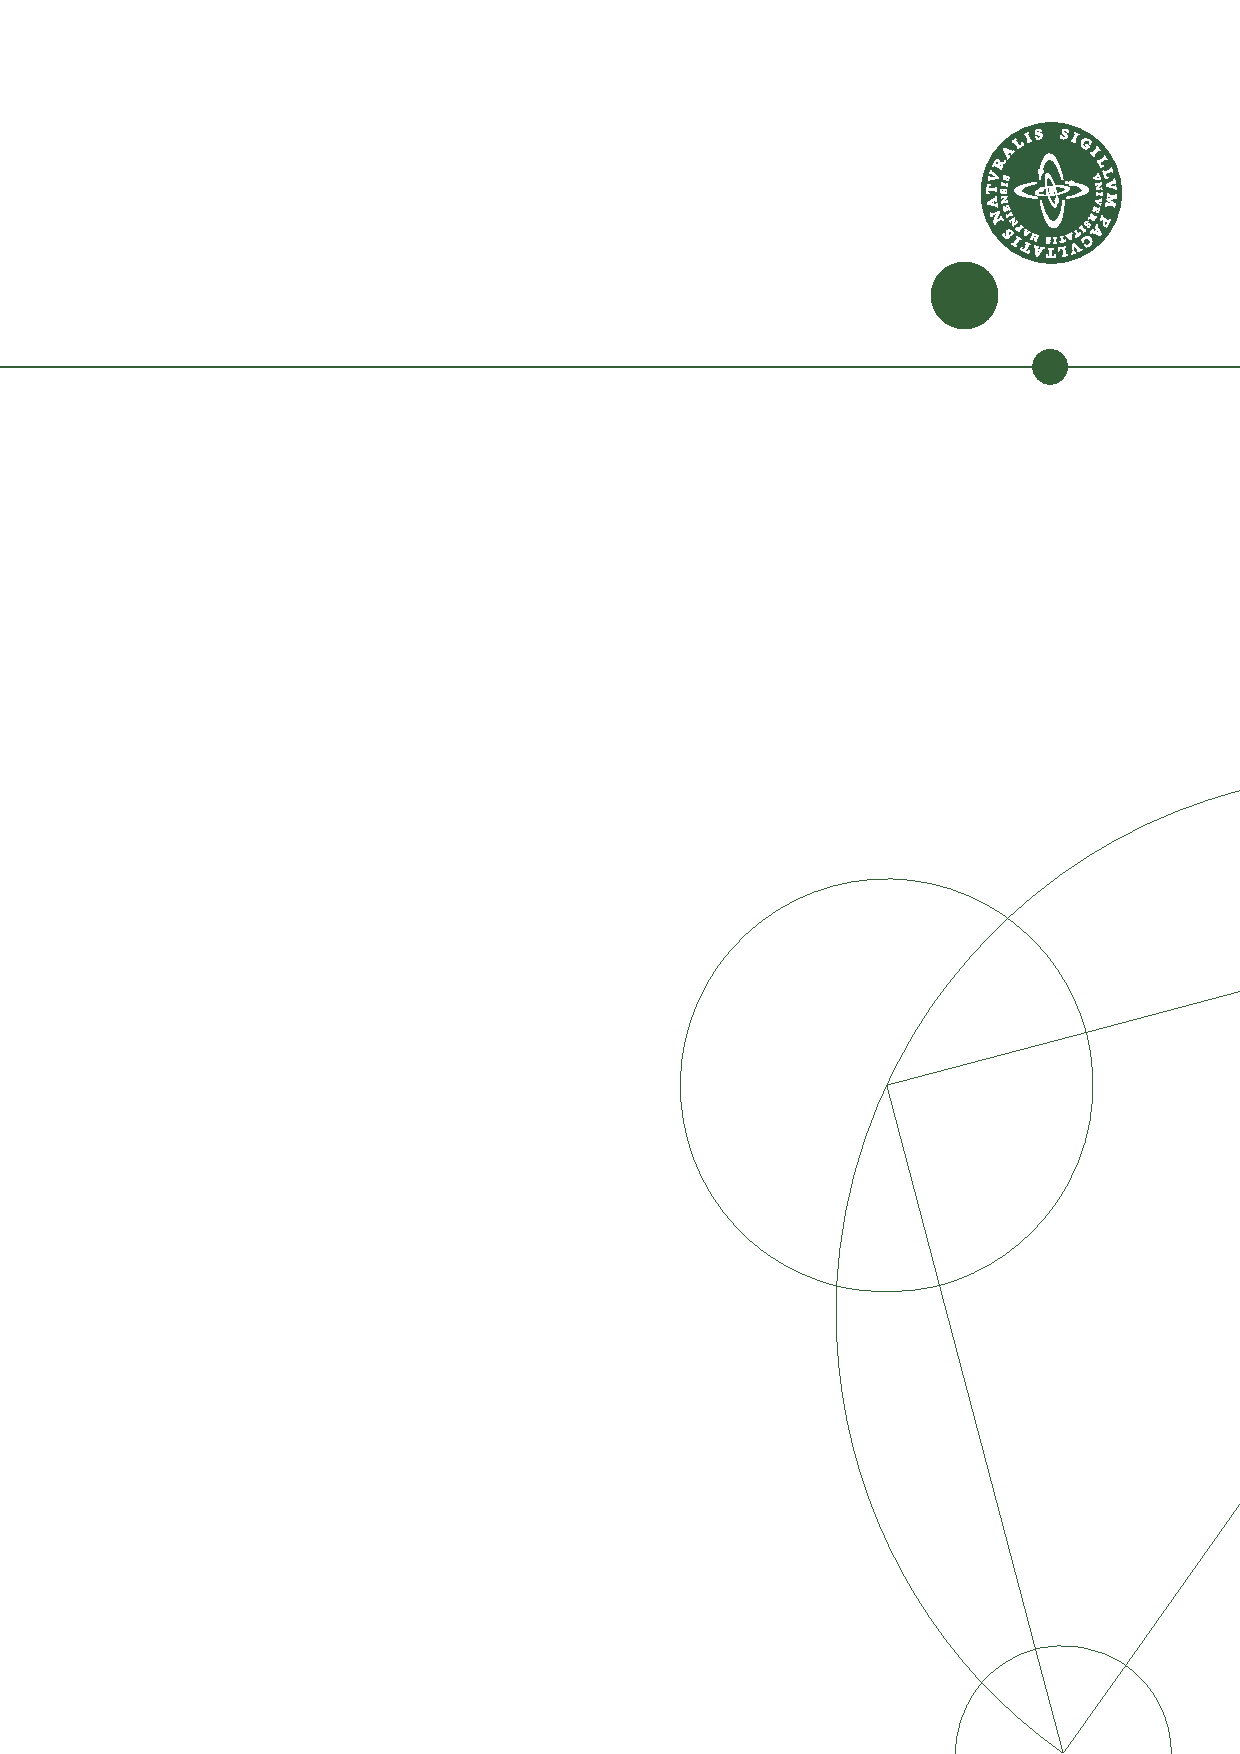
\includegraphics[width=\paperwidth,height=\paperheight]{nat-farve.pdf}}}}

\algnewcommand\True{\textbf{true}\space}
\algnewcommand\False{\textbf{false}\space}
\algdef{SE}[SUBALG]{Indent}{EndIndent}{}{\algorithmicend\ }%
\algtext*{Indent}
\algtext*{EndIndent}

\begin{document} 
	\AddToShipoutPicture*{\BackgroundPic}
	
	\begin{titlepage}
		\thispagestyle{empty}
		\vspace*{5cm}
		\begin{center}
			\Huge \textbf{Diskret Matematik og Algoritmer} \\
			\LARGE \textbf{Aflevering 10g} \\
		\end{center}
		\vspace*{3.5cm}
		\begin{flushleft}
			
		\begin{table}[h!]
			\begin{tabular}{lll}
				Adam Ingwersen,& \\ Aske Fjellerup,&\\ Peter Friborg\\
			\end{tabular}
		\end{table}
			
			
			\vspace{3mm}
			\vspace{3mm}
			Datalogisk  Institut\\
			Københavns Universitet\\
			\vspace{3mm}
			\today\\
			%\vspace*{0.5cm}
			
		\end{flushleft}
	\end{titlepage}

	\title{10g}
	\author{AAP}
	
	\newpage
\newpage

\section{}
\subsection*{a)}
Ved hjælp af logaritmereglerne for et produkt, kan følgende omskrivninger foretages:
\newline
$$
-log(w(e_{1})\cdot w(e_{2})\cdot ... \cdot w(e_{k-1})\cdot w(e_{k}))
$$
$$
-(log(w(e_{1})) + log(w(e_{2})) + ... + log(w(e_{k-1})) + log(w(e_{k}))) 
$$
$$
-\sum\limits_{i=1}^n log(w(e_{i}))
$$
\subsection*{b)}
Her tænkes det at modificere Dijkstra's algoritme via modifikation af \texttt{RELAX} operationen på en \texttt{Edge}. Det er klart, at eftersom at der arbejdes med vægte $w \in {0,1}$, skal der inkoorporeres et multiplikativt element. Det observeres, at \texttt{RELAX} bliver kaldt for hver en \texttt{Vertex} nærliggende en vilkårlig \texttt{Vertex}, v. Hertil anskuer \texttt{RELAX} bagudrettet den bedste (billigste) ved fra v til u som en akkumulation af optimale vertex/edge kombinationer:

\begin{algorithm}[H]
\caption{Modifikation af Dijkstra's algoritme til sandsynligheds-vægte}
\begin{algorithmic}[1]
\Function{Modified Relax}{$u, v, w$}
\State \parbox[t]{.7\linewidth}{if v.d < u.d + log(w(u,v))}
\Indent
\State \parbox[t]{.7\linewidth}{v.d = u.d + log(w(u,v))}
\State \parbox[t]{.7\linewidth}{v.$\pi$ = u}
\EndIndent
\end{algorithmic}
\begin{algorithmic}[1]
\Function{Dijkstra}{$G, w, s$}
\State \parbox[t]{.7\linewidth}{\texttt{INITIALIZE-SINGLE-SOURCE($G,s$)}}
\State \parbox[t]{.7\linewidth}{S = \varemptyset}
\State \parbox[t]{.7\linewidth}{Q = G.V}
\State \parbox[t]{.7\linewidth}{\textbf{while} Q \neq \varemptyset}
\Indent
\State \parbox[t]{.7\linewidth}{u = \texttt{EXTRACT-MAX(Q)}}
\State \parbox[t]{.7\linewidth}{S = S \cup \texttt{{u}}}
\State \parbox[t]{.7\linewidth}{\textbf{for} each vertex v $\in$ G.adj[u]}
\Indent
\State \parbox[t]{.7\linewidth}{\texttt{RELAX($u,v,w$}}
\EndIndent
\EndIndent
\end{algorithmic}
\end{algorithm}

\section{}
\subsection{a)}
Dijkstra's algoritme og BFS i scenariet med enheds-vægte, resulterer i de samme værdier i alle kunder. Dijkstra's anvender en prioritetskø fremfor FIFO-kø (som i BFS), hvorfor Dijkstra's er asymptotisk langsommere end BFS, når w=1. Lad os se, hvorfor disse algoritmer er ækvivalente for w=1:
BFS finder den korteste vej fra s til u - her menes der med den korteste vej, den vej med færrest skridt. Dijkstra's finder den mindst omkostningsfulde vej fra s til u. Hvis omkostningerne for hver \texttt{edge} er ens, vil den korteste vej pr. definition være den billigste. 
\subsection{b)}
I BFS angiver farven \texttt{sort} for en node, at alle nærliggende noder er besøgt. I konteksten for Dijkstra's algoritme, for en node der indgår i sættet S, at denne er blevet tilføjet til mængden S via union af den foregående mængde S og den evaluerede node u, som via \texttt{RELAX} blev vurderet, at være en bedre/billigere node at besøge end den foregående bedste-vej node, v. 
\subsection{c)}
Denne egenskab følger direkte af betingelsen om non-negative \texttt{edges}. 




\end{document}

